\section{Coherent Synchrotron Radiation}

Nowadays, synchrotron radiation facilities, e.g. electron storage rings, are used
to produce intense radiation in wavelength ranges that are not usually reachable
by traditional optical means, in particular in the X-rays and terahertz domain.
This radiation, called synchrotron radiation, is produced when a relativistic electron
is accelerated. In practice, the emission of synchrotron radiation occurs in
the bending magnets or in the undulators of a storage ring.
Relativistic electron bunches circulating in storage rings are used to produce intense
radiation from far-infrared to X-rays. However, above a density threshold
value, the interaction between the electron bunch and its own radiation can lead
to a spatio-temporal instability called microbunching instability. This instability
is characterized by a strong emission of coherent THz radiation (typically 100000
times stronger than the classical synchrotron radiation) which is a signature of the
presence of microstructures (at mm scale) in the electron bunch. This instability is
known to be a fundamental limitation of the operation of synchrotron light sources
at high beam current. \cite{roussel2014}

\tikzexternaldisable
\begin{figure}[H]
	\centering
	\begin{lattice}[0.7]
		\begin{labeldistance}{0.3}
			\cavity{RF cavity}{0.3}[0.6]
		    \drift{0.6}
			\dipole{}{0.6}{45}[][0.4]
			\drift{1.5}
			\dipole{Bending magnet}{0.6}{45}[][0.4]
			\savecoordinate{synch1}[center]
			\drift{1.5}
			\dipole{}{0.6}{45}[][0.4]
			\drift{1.5}
			\dipole{}{0.6}{45}[][0.4]
			\savecoordinate{myCoord1}
			\drift{1.5}
			\savecoordinate{myCoord2}
			\dipole{}{0.6}{45}[][0.4]
			\savecoordinate{myCoord3}[center]
			\drift{1.5}
			\dipole{}{0.6}{45}[][0.4]
			\drift{0.4}
			\setelementcolor{kicker}{cyan}
			\kicker{Undulator}{0.7}
			\drift{0.4}
			\dipole{}{0.6}{45}[][0.4]
			\drift{1.5}
			\dipole{}{0.6}{45}[][0.4]
			\drift{0.6}
		\end{labeldistance}
	\draw[-latex, thick] (myCoord2) -- (myCoord1) node[ellipse, midway, fill=black, minimum width = 10mm] {};
	\draw[draw=none, fill opacity=0, text opacity = 1] (myCoord2) -- (myCoord1) node[midway, above, yshift = 2mm] {$e^{-}$ bunch};
	\draw[-latex, thick, color = red] (synch1) -- ++(-0.5,-1.2) node[near end, color = red, below right] {Synchrotron radiation};
	\draw[latex-, thick] (myCoord3) -- ++(-3.5,0) node[midway, above] {Injection};
	\end{lattice}
	\caption{Basic scheme of an electron storage ring (redrawn from \cite{roussel2014})}
\end{figure}
\tikzexternalenable







\begin{figure}[H]
	\centering
	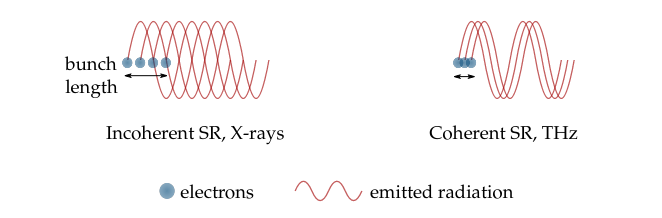
\includegraphics[width = 0.7\textwidth]{chap/02-theory/img/csr2.png}
	\caption{CSR \cite{rota2018}}
	\label{fig:csr}
\end{figure}



\begin{figure}[H]
	\centering
	\includegraphics[width = 0.8\textwidth]{chap/02-theory/img/spectrum.tikz}
	\caption{Electro-Magnetic spectrum}
	\label{fig:spectrum}
\end{figure}





\paragraph{KARA}
\begin{itemize}
	\item Located at the Karlsruhe Institute of Technology (KIT)
	\item Up to 184 electron packages (bunches) can be filled with a distance between two adjacent bunches of \SI{2}{\nano \second}
	\item Operated by the Institute of Beam Physics and Technology (IBPT)
\end{itemize}

\begin{figure}[H]
	\centering
	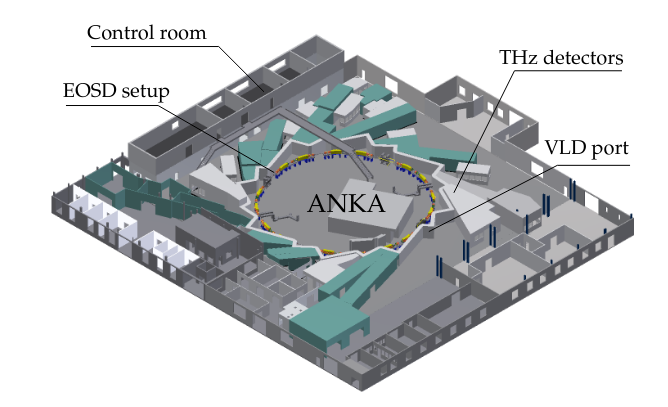
\includegraphics[width = 0.6\textwidth]{chap/02-theory/img/kara.png}
	\caption{Facility \cite{rota2018}}
	\label{fig:kara}
\end{figure}

\subsection{Micro-Bunching Instability}

in the quest for higher emitted synchrotron radiation
power, electron bunches with high charge densities are naturally subject to
a complex nonlinear dynamics which can lead to instabilities. The so-called microbunching
instability or CSR (Coherent Synchrotron Radiation) instability (due
to the interaction of the electrons with their own radiation in bending magnets) is
known to be responsible for the spontaneous formation of microstructures in the
bunch. This spatio-temporal instability is recognized to be a fundamental limitation
of stable operation at high current density in storage rings. In parallel, it
is also considered as a promising source of brilliant THz radiation at high repetition
rate.
\begin{figure}[H]
	\centering
	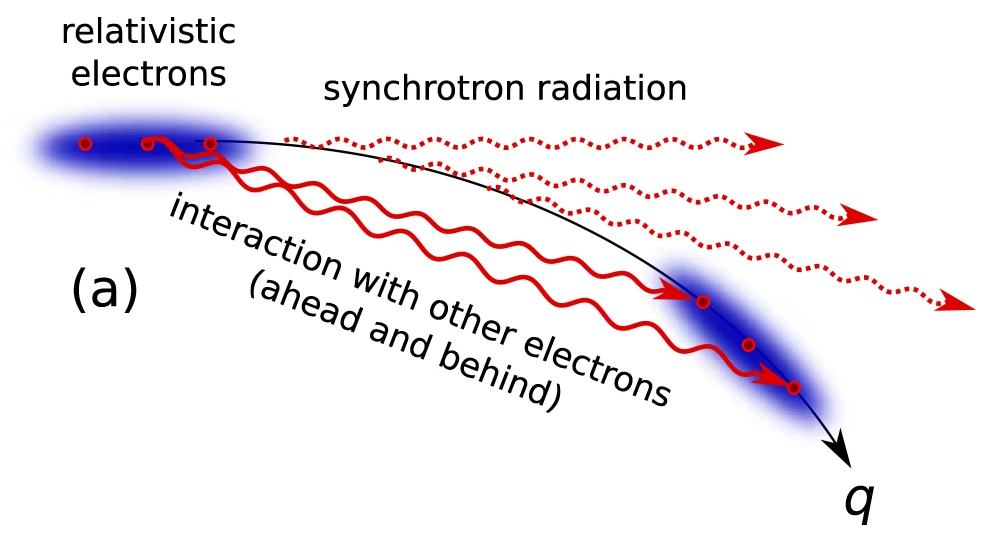
\includegraphics[width = 0.5\textwidth]{chap/02-theory/img/csr.png}
	\caption{Micro-bunching \cite{Bielawski2019}}
	\label{fig:microBunch}
\end{figure}

\newpage 
\section{Photonic time-stretch analog-to-digital converter}










"' In recent and future synchrotron radiation facilities, relativistic electron bunches with increasingly high charge density are needed for producing brilliant light at various wavelengths, from X-rays to terahertz. In such conditions, interaction of electron bunches with their own emitted electromagnetic fields leads to instabilities and spontaneous formation of complex spatial structures. Understanding these instabilities is therefore key in most electron accelerators. However, investigations suffer from the lack of non-destructive recording tools for electron bunch shapes. In storage rings, most studies thus focus on the resulting emitted radiation. Here, we present measurements of the electric field in the immediate vicinity of the electron bunch in a storage ring, over many turns. For recording the ultrafast electric field, we designed a photonic time-stretch analog-to-digital converter with terasamples/second acquisition rate. We could thus observe the predicted link between spontaneous pattern formation and giant bursts of coherent synchrotron radiation in a storage ring. "'  \cite{Bielawski2019}

\begin{figure}[H]
	\centering
	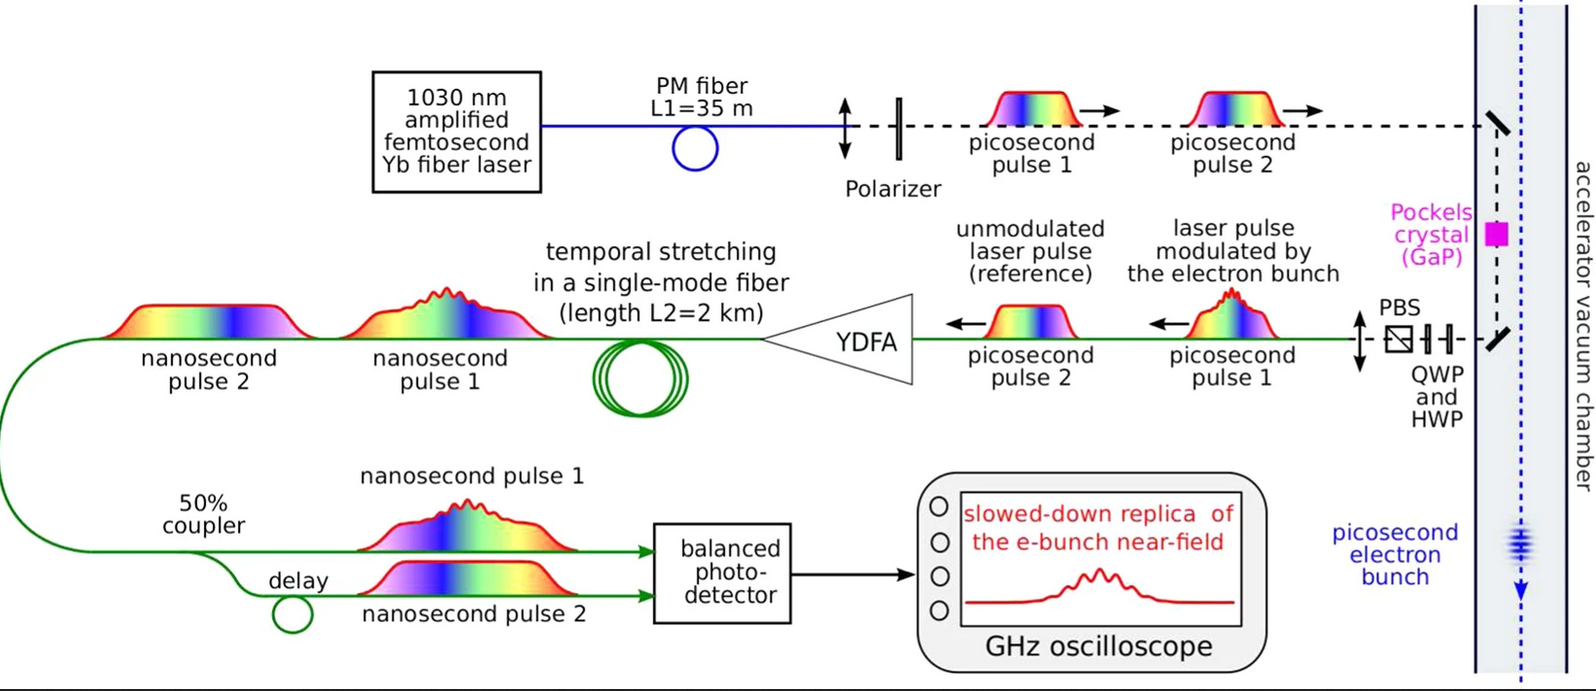
\includegraphics[width = 0.8\textwidth]{chap/02-theory/img/EO.png}
	\caption{Electro-Optical Time-Stretch Technique \cite{Bielawski2019}}
	\label{fig:eo}
\end{figure}


\newpage
\section{Characteristics of Analog-To-Digital-Converters}
Analog-to-digital converters (ADCs) are used to translate analog quantities into digital signals, which can be processed by information processing, computing, data transmission and control systems. This section covers the different characteristics of an ADC, which are needed to evaluate the performance of the developed system. 
\subsection{Sampling Theory}

\paragraph{Nyquist-Criteria}
An ADC samples an analog signal with a frequency $f_s$. This frequency has to be chosen in such way, that the original signal can be fully reconstructed. The Nyquist criteria states, that in order to accurately represent a bandlimited, continous signal
\begin{equation}
y (t) \, \fourier  Y(f) \quad \text{with} \quad Y(f) = 0, \, |f| \geq \frac{B}{2}
\end{equation}
it has to be sampled with a frequency $f_s$ respecting
\begin{equation}
f_s \geq B \quad \text{or} \quad f_s \geq 2 f_a
\end{equation}
with $f_a$ being the highest frequency contained in the signal. \cite{walt} \cite{puente2015}
\paragraph{Sample-And-Hold-Amplifier}
ADCs need a certain amount of time to sample the input signal. If the value of the signal changes by more than one Least-Significant-Bit (LSB) during this period, this can result in large errors in the output signal. Therefore, so called Sample-And-Hold-Amplifiers (SHA) are used in front of ADCs to hold the  input value for the needed amount of time. The ADC sampling needs to be timed in such way, that the analog-to-digital conversion falls into the hold period of the SHA and doesn't exceed into the sample period.



\begin{figure} [H]
\centering
\tikzexternaldisable
\begin{tikztimingtable}
[%
    timing/dslope=0.1,
    timing/name/.style={font=\sffamily\normalsize},
    timing/d/text/.style={font=\sffamily\normalsize},
    grayz/.style={timing/z/.append style={gray}},
    timing/n/.style={rectangle},
    timing/metachar={{K}[2]{#1l !{++(0,+.5\yunit)} N[rectangle,scale=.6]{\shortstack{#2}} !{++(0,-.5\yunit)} #1l}},
    timing/metachar={{J}[2]{#1h !{++(0,-.5\yunit)} N[rectangle,scale=.6]{\shortstack{#2}} !{++(0,+.5\yunit)} #1h}},
  ]
 SHA & 1H 8K{HOLD} 8J{SAMPLE} 8K{HOLD} 3H\\
 Sampling & 5S A 16S A                    \\
\end{tikztimingtable}
\tikzexternalenable
\end{figure}



\subsection{AC errors}
\begin{itemize}
\item Quantization Noise
\item Equivalent Input Referred Noise
\item Noise-Free Code Resolution
\end{itemize}
\paragraph{Integral and Differential Nonlinearity Distortion} 

\paragraph{Dynamic Performance}

\begin{itemize}
\item Harmonic Distortion, Worst Harmonic, Total Harmonic Distortion (THD), Total Harmonic Distortion + Noise (THD + N)
\item Signal-to-Noise-and-Distortion Ratio (SINAD, or S/N + D), Signal-to-Noise ratio (SNR), Effective Number of Bits (ENOB)
\item Analog Bandwidth (Full-Power, Small-Signal)
\item Spurious Free Dynamic Range (SFDR)
\item Two-Tone Intermodulation Distortion, Multi-Tone Intermodulation Distortion
\item Noise Power Ratio (NPR)
\item Adjacent Leakage Ratio (ACLR)
\item Noise Figure
\item Setting Time, Overvoltage Recovery Time
\end{itemize}

\cite{walt}
\subsection{Interleaving}

\begin{itemize}
\item Net sample rate
\item Interleaving Spurs
\end{itemize}

\cite{mangrob}
%\begin{figure}[H]
%	\centering
%	\includegraphics[height = 0.3\textwidth, width = 0.6\textwidth]{chap/03-work/img/pll_karaMode.tikz}
%	\caption{PLL in "KARA-mode"}
%	\label{fig:pll}
%\end{figure}



\newpage
\section{RF/Microwave Design Basics}